\documentclass[12pt,letterpaper]{article}

\usepackage[utf8]{inputenc}
\usepackage[margin=1in]{geometry}
\usepackage{setspace}
\usepackage{amsmath}
\usepackage{graphicx}
\usepackage{hyperref}
\usepackage{natbib}
\usepackage{titlesec}
\usepackage{abstract}

\doublespacing

\title{The Mystery Machine: A Classroom Investigation of the Cognitive Processes Underlying Instructionless Learning}
\author{Jeff Shrager}
\date{}

\begin{document}

\maketitle

\begin{quote}
\textbf{``The Homework Machine, Oh, the Homework Machine, Most perfect contraption that's ever been seen...''} \\
--- Shel Silverstein
\end{quote}

\begin{abstract}
Instructionless Learning is the process of figuring out an unfamiliar setting without being told. It is the more commonplace cousin of exploratory learning and scientific discovery, and is one of the most familiar and efficient ways people learn in everyday settings. I describe a classroom activity that enables students to observe and analyze instructionless learning at the cognitive level. Learners must figure out how to operate a slightly puzzling device, called the Mystery Machine, through observation, experiment, and reasoning. By observing a learner struggle to figure out the Mystery Machine, students learn about the cognitive operators that guide Instructionless Learning, and about the cognitive operators learners deploy in such settings, and about the gradual construction of "mental models" -- the knowledge that enable us to reason effectively in complex settings.
\end{abstract}

\section{Introduction}

All of us are familiar with having had to figure out a new gadget or setting, for example, an new app, a rental car, a new checkout system at the store, how to order in a new restaurant, a new social setting, and so on. We are remarkably good at this kind of spontaneous "figuring out" -- a cognitive skill that is more technically called ``Instructionless Learning''\cite{shrager1986instructionless}. 

Instructionless learning is neither mere guessing, nor is it as precise as scientific reasoning. Learners efficiently build and refine their knowledge of how the setting works and how to interact with it, through repeated cycles of observation, hypothesis formation, experimentation, explanation, and evolution of their knowledge about the setting.\footnote{In this article, I will use the vague terms "model" (sometimes "mental model"), "understanding", and "knowledge" interchangeably.} This article describes an in-class experiment where learners are observed figuring out a puzzling device called the Mystery Machine. The activity was developed for Symbolic Systems 245, a senior applied cognition seminar at Stanford University. Over more than two decades hundreds of Stanford students have participated in it. The Mystery Machine is designed to be a little bit difficult and a little bit confusing, so that learners need to work a bit at figuring it out, but it is not so complex as to be frustrating. This balance enables students to analyze how the learners deploy Instructionless Learning.

\section{The Mystery Machine Exercise}

The present exercise adapts classic work by David Klahr and colleagues\cite{klahr2000exploring}. The Mystery Machine itself (which we shall hereafter call just "MM", Figure \ref{fig1}, \cite{MMRepo}) is browser-based. The exercise can be run in about an hour, including discussion. Students will directly observe the cognitive operators people use when figuring out novel systems, understand how mental models form and evolve during learning, develop skill in observing complex cognitive activity in themselves and others, recognize the opportunistic, and learn about important cognitive processes including explanation and mental model evolution.

\section{Procedure}

\subsection{Phase 1: Learning the MM Basics}

Students form small groups. Each group opens one copy of the MM on one of their browsers. It comes up in "Phase 1: Learn the Mystery Machine." In the interest of space, and getting to the intresting second phase of the exercise I don't explain the MM here. I assume that whoever is guiding the exercise will have studied it before the session, and can explain it clearn to the students. I suggest guiding the class through this Phase so that within about ten minutes, they are proficient with the basic command entry, and what to expect. I also suggest using the displayed keypad explclusiovely, for most of it, but that at the end showing that they can do the same thing using their keypad. They should also experience pressing [Save History] at least once times so that they know how to save the history, and know where it is being saved.\footnote{Except for the very end of the exercise, this is mostly done automatically, but it's worth trying in this phase so that when it happens automatically the file-saving pop-up isn't a surprise, and because they will need to do it manually at the very end of the exercise.} 

\begin{figure}[!htb]
    \centering
      \makebox[\textwidth]{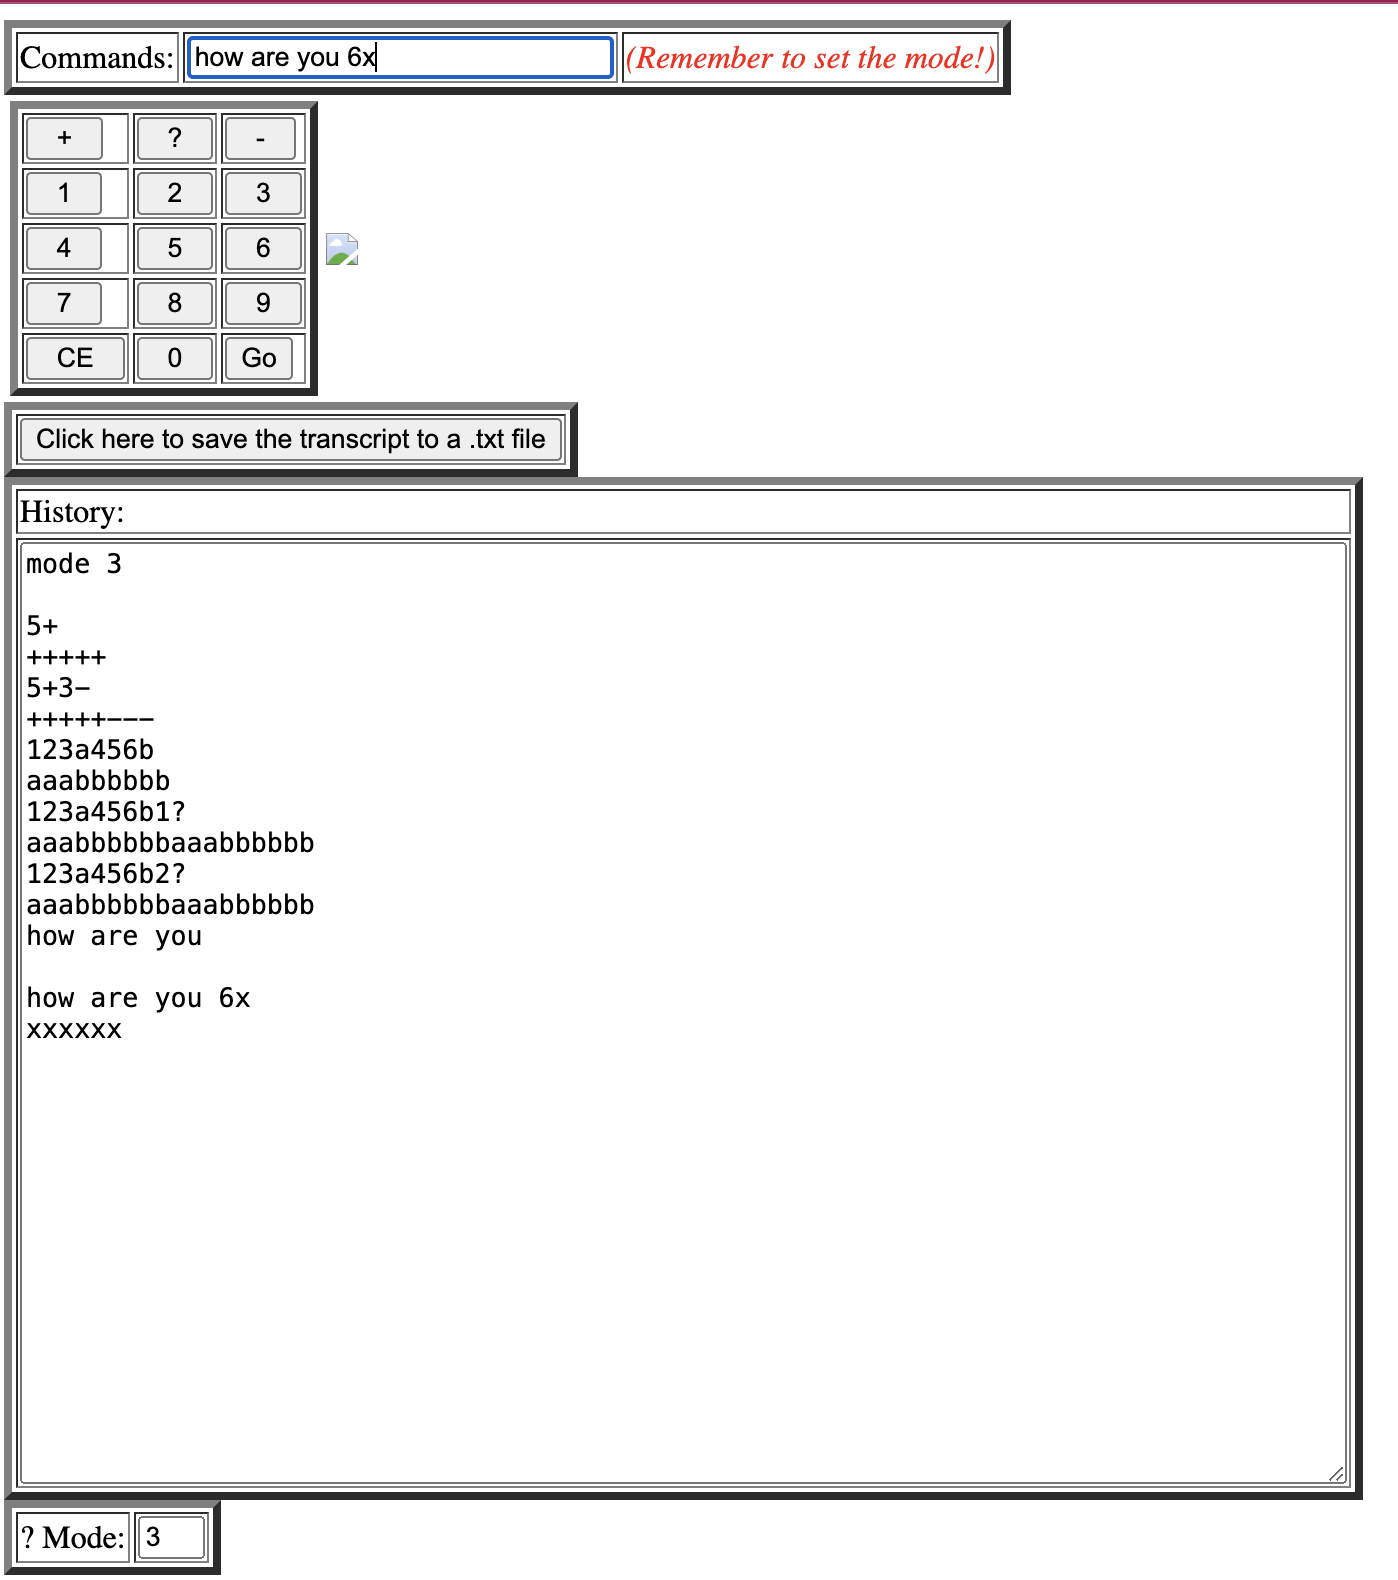
\includegraphics[width=\textwidth]{btlab1.png}}
        \caption{MM Interface Screenshot}
    \label{fig1}
\end{figure}

Note that the MM is \textit{intentionally} designed to be somewhat confusing. The importance of this will become clearer when we get to the discussion. Here are some of the confusions that might arise: \textbf{Plus and minus are misleading:} Despite appearances, the MM is \textit{NOT} a calculator. The ``$+$'' and ``$-$'' are just characters like any other. ``$5+1$'' produces ``+++++'' (five pluses), NOT ``$6$'' or ``$++++++$'' (six pluses). \textbf{Multiple pluses and minuses are hard to distinguish:} Here is the same program as just above, but using minuses instead of pluses: ``$5-1$'' or ``$------$''. Could you tell that I put 6 minuses instead of 5? \textbf{Only the last digit matters:} The MM has a single-digit ``register'' that overwrites with each new digit. If you enter ``$12343247+$'' the output is ``$++++++++$'' (seven plus signs), because only the final ``$7$'' is retained. \textbf{No error checking:} Malformed programs still execute, often producing confusing results. For example, ``$3-+$'' produces ``$- - - +++$'' because the $3$ applies to both the minus and the plus sign. 

\textbf{A path to less confusion: Alternative characters work equally well:} ``3x4y'' produces ``xxxyyyy'' just as well as ``3+4-''. Once explorers discover this, they can avoid the confusing plus/minus characters, though many don't discover it on their own. I've found that it is useful to mention this in passing, but not emphasize it; explorers in phase 2 who are being confused by the minuses may recall that this is possible and use it spontaneously, but it's useful for them to experience some of the above-described difficulties before learning that they can avoid some of them by using x's and y's (or other characters of their choice).

\textbf{Phase 2: Figuring Out the ? Key}

Each team now chooses an initial "explorer". The task of the explorer is to try to figure out what the ? key does, as explained in more detail below. To begin, click the button called [Move to Phase 2]. This button will disappear and a mode will be displayed. The mode is initially set to 3.

The explorer can type anything they like using either the MM displayed keypad, or the computer keyboard (except, of course, to change the mode or to otherwise ruin the experiment). The task of the rest of the team in this phase is to keep the explorer talking about what they are doing -- ask them what they are thinking. I find it useful to give each explorer only 5 minutes, and then, if the current explorer hasn't figured out the current mode, rotat the explorer role. Also rotate the explorer role once the team (that is, the current explorer) figures out the current mode (or the team gives up).

Once the explorer has either discovered the ? function, or given up so that the function is revealed by the facilitator, the group changes mode. I recommend this sequence: Mode 3 $\rightarrow$ Mode 4 $\rightarrow$ Mode 6 $\rightarrow$ Mode 2 $\rightarrow$ Mode 1 $\rightarrow$ Mode 5 (if you dare!). Note that the MM will try to save the input output trace to a local file; This will be useful in discussion, so agree in advance as to where these will be saved and named.  

Generally I let this go on for about 20 minutes, leaving about 20 minutes in a one hour class session for discussion.

\subsection{What the ? Key Actually Does}

Here is what the ? key does in each mode. ``\#'' refers to the digit before the ? (or anyway whatever the most recent digit was). 

\begin{itemize}
\item \textbf{Mode 3} (simplest): Repeats the entire program once, regardless of the numerical prefix. 
\item \textbf{Mode 4}: Restarts at the \#th \textit{step} (digit-character pair).
\item \textbf{Mode 6}: Restarts \# \textit{steps} back from the ?
\item \textbf{Mode 2}: Restarts at the \#th \textit{character} position (where the first character is \#1).
\item \textbf{Mode 1}: Restarts \# \textit{characters} back from the ?
\item \textbf{Mode 5}: Restarts at a \textit{random character position} (non-deterministic!)
\end{itemize}

Aside from Mode 3, which is fairly simple, these can be extremely confusing. Modes 4 and 6, for example, refer to "steps", meaning digit-character pairs, where the first pair is step \#1, and so on. To do this, the MM skips two characters at a time through the program to the desired point. For example, if the program is "3x2y1z", and you add 3? in mode 4, that is: "3x2y1z3?" the result will be "xxxyyzz" because the program skipped to location 5 -- the character at which the 3rd step begins. This is find, if the program is in "standard form" -- that is, a series of digit-character pairs, as above. But recall that the MM does not check that the entry is in standard syntax, and it is quite common for explorers to be careless about this, making these modes \textit{very} confusing.\footnote{It may be useful for the facilitator to remind the explorer to use standard syntax, if they are not already, and are becoming confused as a result.} So, for exmaple, if one were to put space between one's steps, as: "3x 2y 1z 3?", the result would be: "xxx   yy  z yyy   z". I leave it as an exercise for the reader to figure out why this output is correct for mode 4 (hint, it starts at the same \textit{character position} as in the correct example, above). 

Modes 2 and 1 are even more confusing because they interpret the argument as an instruction start at a particular character position in the previous body of the program, not on a particular step. Therefore, the results of the previous examples in mode 2 are: "3x2y1z?3"
-> "xxxyyzxyyz", and "3x 2y 1z 3?" -> 
"xxx   yy  z yy  z". Again, we leave it to the reader to figure out why.

Another thing that the facilitator might mention if the explorer is becoming confused is to encourage them to think about what the number before the ? might be referring to. 

This set of examples provides an opportunity to observe another very intersting, and somewhat annoying, "feature" of the MM. Note the subtle difference between the two second sets of outputs: "xxx   yy  z yyy   z" v. "xxx   yy  z yy  z" Even though you may have noticed that there is an extra 'y' in the first output, you probably didn't notice that there is also an extra space before the final 'z'. Later, in the discussion we'll return in some detail to this seemingly trivial, but in fact deep and revealing common misreading. 
===============================
\section{Discussion Part 1: The Shape of Instructionless Learning}

\subsection{The 8E's: Core Cognitive Operators in Instructionless Learning}

Instructionless Learning is a problem solving activity define, as is all human problem solving, by a goal and operators -- cognitive or physical actions that change the problem state, eventually (hopefully) reaching the goal\cite{simon_newell1972_human_problem_solving}. Here the goal is a correct understanding of the ? key for a particular mode. We shall describe eight operators -- what I call ``The 8 E's'' -- that explorers usually use to reach this goal. However, before studying these operators, it is important to understand that human problem solving is fundamentally \textit{opportunistic}, that is, it doesn't follow a rigid sequence. No two explorers will reach the goal in the same way, and the specific order in which operators are used by a given explorer in a given setting depends on countless factors, such as what the explorer notices, what they happen to try, what confusions they encounter, and what knowledge they bring to the setting. Although we will present the 8 operators in a particular order, and there seems to be a natural order to some of them, there is no hard-and-fast rule that says what order these must appear in during the course of figuring out what the  MM's ? key does.

The 8 E's are:

\begin{itemize}
\item \textbf{Exploration} - trying things without specific expectations
\item \textbf{Evidence} - gathering outputs and observations
\item \textbf{Explanation} - making sense of the evidence based on one's current model
\item \textbf{Experimentation} - testing specific hypotheses
\item \textbf{Expectation} - predicting what should happen
\item \textbf{Evaluation} - assessing whether results match expectations
\item \textbf{Evolution} - updating mental models based on findings
\item \textbf{Exercise} - practicing once a correct (or presumed correct) model is achieved

\end{itemize}

While describing these I ask the class to think of examples of these operators that they saw in their own protocols. 

\subsection{The Typical Arc of Figuring Things Out}

When first confronted with the ? key, some explorers may simply guess at its function. They may even guess correctly, although they still need to run experiments to confirm that they are correct. More commonly, explorers begin with \textbf{Explorations}—trying several programs containing ? with only vague \textbf{Expectations} of what might happen. They gather \textbf{Evidence} (the outputs), then engage in \textbf{Explanation}, usually forming a preliminary mental model.

To validate this model, they run \textbf{Experiments} with more specific \textbf{Expectations}. They again gather \textbf{Evidence}, but now they \textbf{Evaluate} it against their predictions. If the \textbf{Evaluation} succeeds -- the evidence matches (or apparently matches) their expectation -- they may declare victory and move to \textbf{Exercise}—using their understanding playfully.

If \textbf{Evaluation} fails, explorers face a choice. They might try to \textbf{Explain} the mismatch between their expectaion and the evidence; they might discard their expectation and return to try to \textbf{Explain} the evidence behavior independently of the failed expectations; They might return to \textbf{Exploration}, seeking new evidnence; or they might reject the experiment as poorly designed. Of coure at any point the explorer might simply give up! (Perhaps this should be the 9th "E": Exit!)

When explanation leads to mental model \textbf{Evolution}, the cycle begins again with new \textbf{Experiments} based on the revised model, until the leaner decides that they are satisfied that they have a correct model, at which point (as above) they fall into exercises.  

\subsection{The 8 E's in More Detail}
\subsubsection{Exploration: Poking Around Without a Plan}

\textbf{Students will observe} that subjects often begin by just trying things. An Exploration differs from an Experiment in stance and expectation. In Exploration, the goal is simply to gather \textbf{Evidence} without a specific prediction of what will happen.

\textbf{Example from a protocol:}
\begin{quote}
``I'm just going to try something... okay, let's see... 3x2?'' [Types it, clicks GO]

``Okay, that gave me... xxxxxxxx. Huh. So it did something.''
\end{quote}

Notice the explorer isn't testing a specific hypothesis; they're fishing for data that might suggest a hypothesis.

\subsubsection{Evidence: Gathering Information}

Every interaction with the MM produces \textbf{Evidence}—the output displayed on screen. However, \textbf{students will observe} that evidence gathering isn't as simple as just reading what appears. Subjects often:

\begin{itemize}
\item \textbf{Miscount} the output (especially with + and -)
\item \textbf{Misremember} what they typed
\item \textbf{Fail to notice} important patterns
\item \textbf{See what they expect} rather than what's there (expectation bias)
\end{itemize}

This is why the MM intentionally uses confusing characters. Long strings like ``++++++------'' are hard to count accurately, leading to interesting errors.

\subsubsection{Expectation: What Should Happen?}

\textbf{Expectations} come in two varieties:

\textbf{Vague expectations} (typical of Exploration): ``Something will happen and I'll learn from it.''

\textbf{Specific expectations} (typical of Experiments): ``This program should produce exactly this output.''

\textbf{Students will observe} that the specificity of expectations dramatically affects how explorers respond to results. A vague expectation means almost any output is ``interesting,'' while a specific expectation creates a clear success/failure criterion.

\subsubsection{Evaluation: Did It Match?}

After gathering \textbf{Evidence}, explorers \textbf{Evaluate} whether it matched their \textbf{Expectation}. 

\textbf{Students will observe} that evaluation seems trivial but isn't:

\begin{itemize}
\item During \textbf{Exploration}, evaluation is loose—subjects are satisfied if they learned something
\item During \textbf{Experiments}, evaluation should be rigorous—but often isn't
\item \textbf{Expectation bias} can cause subjects to ``see'' what they expected even when it's not there
\item \textbf{Near misses} often get accepted as successes
\end{itemize}

\textbf{Example of failed evaluation:}
\begin{quote}
``So if I do 4x2? that should give me... wait, how many x's is that? Let me count... okay, xxxxxxxx, that's eight. So it doubled it! I think it repeats the command.''

[The subject miscounted—it was actually twelve x's, not eight. They've formed an incorrect theory based on miscounting.]
\end{quote}

\subsubsection{Explanation: Making Sense of It All}

\textbf{Explanation} is perhaps the most interesting and least understood operator. When subjects try to explain what the ? key does, they're drawing on:

\begin{itemize}
\item The \textbf{Evidence} they've gathered
\item Their background knowledge (calculators, programming, math)
\item Their current mental model of the MM
\item Analogies and intuitions
\end{itemize}

\textbf{Students will observe} that explanations come in many forms:

\textbf{Early explanations} (after Exploration):
\begin{quote}
``I think it does something with the number before it... maybe it repeats?''
\end{quote}

\textbf{Mid-stream explanations} (after failed Experiments):
\begin{quote}
``Okay, so it's not just doubling... maybe it's adding the number to the command? No, that doesn't make sense either...''
\end{quote}

\textbf{Confident explanations} (after successful Experiments):
\begin{quote}
``Oh! It's going back to the beginning and doing the whole thing again!''
\end{quote}

Explanation is deeply tied to a process I'll call ``interpretation'' or ``view application,'' which we'll explore in depth in Discussion Part 2.

\subsubsection{Experimentation: Testing Specific Ideas}

Once explorers have a theory (from \textbf{Explanation}), they often design \textbf{Experiments} to test it. An \textbf{Experiment} differs from \textbf{Exploration} in having:

\begin{itemize}
\item A specific hypothesis under test
\item A specific \textbf{Expectation} of the outcome
\item A clear criterion for \textbf{Evaluation}
\end{itemize}

\textbf{Students will observe}, however, that subjects are often quite poor at designing good experiments. Common problems include:

\textbf{Non-discriminating experiments:} Tests that don't distinguish between theories.

\textbf{Example:} If the explorer thinks ``?'' repeats the whole program, they try ``2+1?'' expecting ``++++''. But this result is also consistent with ``? doubles the last command,'' ``? adds 2 to everything,'' and many other theories.

\textbf{Overly complex experiments:} Tests too complicated to interpret.

\textbf{Example:} 
\begin{quote}
``Let me try 12x34y56z78?'' [Types it]

``Okay, that gave me... wait, what did I even expect this to do?''
\end{quote}

\textbf{Confounded experiments:} Tests where multiple things changed at once.

Despite these limitations, subjects usually succeed eventually—more on why in the ``Satisficing'' section below.

\subsubsection{Exercise: Playing With Understanding}

Once subjects believe they understand the ? key, their stance shifts from testing to using. \textbf{Students will observe} this shift in verbalizations:

\textbf{During Experimentation:}
\begin{quote}
``If my theory is right, this should produce...''
\end{quote}

\textbf{During Exercise:}
\begin{quote}
``Okay, now let me make it do something cool... how about a pattern?''
\end{quote}

\textbf{Exercises} often have \textbf{Expectations}, but subjects are less rigorous about \textbf{Evaluation}. They're confident enough that small discrepancies get ignored. This is why subjects often declare success even with partially incorrect models.

\subsubsection{Evolution: Updating the Mental Model}

When \textbf{Evaluation} reveals that \textbf{Evidence} doesn't match \textbf{Expectation}, explorers must decide what to do. The most productive response is \textbf{Evolution}—updating their mental model to account for the new data.

\textbf{Students will observe} several patterns:

\textbf{Incremental evolution:} Small tweaks to the existing model.
\begin{quote}
``Okay, so it doesn't repeat just once... maybe it repeats the number of times in the argument?''
\end{quote}

\textbf{Revolutionary evolution:} Complete model replacement.
\begin{quote}
``Wait, I've been thinking about this all wrong. It's not repeating commands—it's moving backward in the program!''
\end{quote}

\textbf{Evolution through impasse:} Sometimes subjects get completely stuck, stare at the results, and suddenly have a breakthrough.
\begin{quote}
[Long silence]

``Oh! OH! I get it! It's not counting characters, it's counting the PAIRS!''
\end{quote}

The process underlying evolution—how subjects integrate new information to revise their understanding—involves what I call ``interpretation,'' explored in depth in Discussion Part 2.

\subsection{Key Observations About the 8E's}

Having introduced all eight operators, students should now annotate their transcripts, labeling each segment with the relevant E. Usually, every line of a think-aloud protocol can be assigned to one or more operators.

Some key discussion points:

\textbf{1. The operators don't follow a fixed sequence.} A explorer might go: Exploration $\rightarrow$ Explanation $\rightarrow$ Experiment $\rightarrow$ Evaluation $\rightarrow$ Exploration $\rightarrow$ Explanation $\rightarrow$ Exercise. Or any other path. This opportunism is fundamental to human cognition.

\textbf{2. Some operators are really methods themselves.} Explanation, for instance, is highly complex and draws on many cognitive processes. There's no bright line between ``operators'' and ``methods.''

\textbf{3. Evaluation and evidence-gathering blur together.} What you expect influences what you see. This is expectation bias, and it's everywhere in the protocols.

\textbf{4. Evolution is both the goal and the least understood operator.} We'll unpack it more in Discussion Part 2.

\section{Satisficing: Why Imperfect Problem-Solving Succeeds}

At this point, students might notice a paradox: \textbf{Subjects are simultaneously very good and very bad at figuring things out.} They're \textbf{good} at eventually reaching correct (or mostly correct) understanding. They're \textbf{bad} at designing optimal experiments, carefully evaluating evidence, avoiding expectation bias, and systematically forming and testing hypothesis.

So why does instructionless learning work at all?

\subsection{Explorers Satisfice Efficiently}

Herbert Simon, the Nobel laureate who is usually credited with having founded cognitive science, introduced the concept of \textbf{satisficing}—accepting a solution "that will permit satisfaction at some specified level of all of [the explorer's] needs." rather than searching for the optimal one. This is a consequence of \textbf{bounded rationality}: humans have limited time, knowledge, and cognitive capabilities (\cite{Simon1956}, p.136).

\textbf{Students will observe} that subjects don't design perfect experiments—they try something reasonable; don't exhaustively test hypotheses—they run a few trials and move on; don't carefully analyze all past evidence—they focus on recent observations; and don't eliminate all alternative theories—they accept ``good enough'' \textit{This is actually smart}, not stupid! The stakes are low, data is cheap and fast to collect, and subjects aren't professional scientists. The MM environment rewards trying a lot of simple things rapidly, rather than than careful systematic investigation.

There are many settings where satisficing results in much more thoughtful and careful behavior. Consider scientists trying to create cancer drugs. In that setting experiments cost millions of dollars, results take years to obtain, effect sizes are tiny, and human lives depend on getting it right. Drug scientists spend years on preliminary work before human trials. They must design optimal experiments because the cost of poor experiments is measured in human suffering. The MM is the opposite extreme: experiments are free, instantaneous, and low-stakes; trying lots of simple experiments and not worrying about designing them carefully, nor about interpreting the results perfectly, is a good strategy here.\footnote{Klahr and Dunbar (1988) described instructionless learning as ``dual-space search'' where explorers simultaneously search a \textbf{space of experiments} and a \textbf{space of theories}. Although this model is useful for understanding the overall shape of learning, it assumes explorers can reliably create good experiments (they can't); that explorers reliably interpret results (they don't). It also doesn't account for satisficing and doesn't explain how theories actually evolve (the interpretation problem).}

\section{Discussion Part 2: How Mental Models Form and Evolve}

Having explored \textbf{what} explorers do (the 8E's), we now examine \textbf{how} understanding emerges. This requires delving into mental models, interpretation, and the mysterious process of ``view application.''

\subsection{What Is a Mental Model?}

Throughout this discussion, we've said explorers ``understand'' the MM or ``figure out'' what the ? key does. But what does ``understand'' actually mean?

\textbf{Students should recognize} that ``understanding'' is remarkably vague and domain-specific:

\begin{itemize}
\item A teenager might say to their parents, ``You just don't understand me''
\item A mechanic might say they ``understand'' what's wrong with your car
\item Your subject came to ``understand'' the ? key
\item Students came to ``understand'' how the MM works when learning it
\item You might gain an ``understanding'' of what understanding means by reading this paper
\end{itemize}

In each case, ``understanding'' means roughly: \textit{having whatever knowledge, skills, and problem-solving ability you need to achieve your goals in this domain.}

For MM subjects:
\begin{itemize}
\item Goals: Design programs that use the ? key effectively
\item Understanding: Knowledge of what ? does in each mode, plus ability to write and predict program behavior
\end{itemize}

\textbf{Importantly:} Being correct isn't required for understanding. An incorrect understanding is still an understanding. Many subjects confidently declare they've figured it out when their theory is wrong—but their theory is detailed enough to generate programs and predictions, so they have achieved \textit{an} understanding, even if not \textit{the correct} understanding.

\subsection{Mental Models Enable Goal Achievement}

A mental model is whatever internal representation enables you to reach your goals with a system. These goals might be:

\begin{itemize}
\item Operating the system
\item Reasoning about it
\item Explaining it to others
\item Predicting its behavior
\item Designing inputs to produce desired outputs
\end{itemize}

Different goals require different mental models. An MM subject needs enough model detail to write programs. An experimenter teaching a subject needs a model detailed enough to explain and demonstrate. A designer creating a new MM mode needs a model of the underlying code.

\subsection{The Three E's of Understanding: Evaluation, Explanation, Evolution}

Five of the 8E's (Exploration, Experimentation, Expectation, Evidence, Exercise) describe the \textbf{shape} of instructionless learning—what explorers do and when. But three E's—\textbf{Evaluation, Explanation, and Evolution}—describe the \textbf{content} of learning: how mental models actually form and change.

These three are deeply intertwined with a fundamental cognitive process called \textbf{interpretation}.

\subsection{Interpretation: The Foundation of Understanding}

\textbf{Students will observe} that subjects often have moments of sudden insight:

\begin{quote}
``Oh! I get it!''

``Wait... ohhhhh.''

``NOW I see what it's doing!''
\end{quote}

These moments signal mental model evolution. But what actually happens in these moments?

The answer involves a cognitive process that operates largely below conscious awareness. I call this process \textbf{``view application''} or \textbf{``commonsense perception.''} Understanding this process is crucial because it doesn't just operate in the MM—it operates constantly, in every domain of human activity.

\subsection{View Application: A Ubiquitous but Mysterious Process}

View application (VA) is so ubiquitous that it's been discovered and redescribed many times under different names:

\begin{itemize}
\item Minsky called it ``framing''
\item Schank called it ``script matching''
\item Fauconnier called it ``conceptual blending''
\item Gentner calls it ``analogy''
\item Hampton calls it ``conceptual combination''
\end{itemize}

All these researchers discovered approximately the same cognitive process operating in different contexts. What does VA do? \textbf{It updates your overall cognitive state—including your mental models—in light of new information.}

\subsection{Seeing VA in Action: The Sixth Sense Example}

Let me demonstrate VA with an example students can experience directly:

\textbf{Version 1:} I was on the east coast last week giving a talk, and I got to the hotel and there was a bug in the room. Ugh!

\textbf{Version 2:} I was in DC last week giving a talk at the CIA, and I got to my room and there was a bug in the room!

\textbf{Students should notice} that they got a different sense of ``bug'' in the two versions. Version 1: an insect. Version 2: a listening device. Your understanding of ``bug'' was different because the context (CIA) triggered a different interpretation.

This reinterpretation happened instantly, automatically, and completely changed the meaning of everything around it. That's view application.

\subsection{The ``Oh I See'' Phenomenon}

Consider the joke:

\begin{quote}
A rabbit, a priest, and an imam walk into a blood bank. The priest says, ``I'm a type A.'' The imam says, ``I'm a type B.'' And the rabbit says, ``I'm a type O.''
\end{quote}

The moment you ``get it''—when you realize ``type O'' sounds like ``typo''—that's VA in action. Your mental model of what's happening in the joke completely restructures.

Or consider \textit{The Sixth Sense}: throughout the movie, you think Bruce Willis is alive. At the reveal, you suddenly realize he's been dead the whole time. If you rewatch the movie, you see a completely different movie—every scene reinterpreted through your new understanding.

\textbf{This reframing process is VA.} It operates constantly:

\begin{itemize}
\item Every word you read triggers VA
\item Every conversation requires VA
\item Every attempt to figure something out involves VA
\item The MM subject saying ``Oh! It's a loop!'' is doing VA
\end{itemize}

\subsection{VA in the Mystery Machine}

\textbf{Students will observe} VA operating throughout their protocols:

\textbf{Early VA:} ``Oh, it's like a calculator!''
\begin{itemize}
\item The subject applies the ``calculator'' view, shaping all subsequent interpretation
\end{itemize}

\textbf{Mid-stream VA:} ``Wait, it's not a calculator... it's more like programming?''
\begin{itemize}
\item The ``programming'' view replaces the calculator view
\end{itemize}

\textbf{The ? key breakthrough:} ``Oh! It's repeating the whole program!''
\begin{itemize}
\item A ``loop'' view gets applied to explain the ? behavior
\end{itemize}

Each of these moments involves VA—the subject taking an abstract concept (calculator, program, loop) and applying it to reformulate their understanding of the MM.

\subsection{Why ``Commonsense Perception''?}

I prefer ``commonsense perception'' to ``view application'' because:

\textbf{Commonsense:} The views being applied are everyday concepts—calculators, programs, loops, repetition—not technical abstractions. They're grounded in common experience.

\textbf{Perception:} Although this isn't literal sensory perception, it shares key properties:
\begin{itemize}
\item It happens rapidly and often unconsciously
\item It's holistic—understanding shifts all at once
\item It's grounded in experience
\item It enables recognition and understanding
\end{itemize}

The phrase ``I see what you mean'' captures this perfectly—understanding feels like seeing, even though nothing visual is happening.

\subsection{Evolution Through Interpretation}

So how do mental models actually \textbf{evolve}? Through repeated cycles of interpretation:

\begin{enumerate}
\item explorer has mental model M1
\item Evidence E arrives that doesn't fit M1
\item explorer applies view V to reinterpret M1 and E together
\item New mental model M2 emerges from this interpretation
\item Cycle repeats
\end{enumerate}

\textbf{Students will observe} this cycle repeatedly:

\begin{quote}
``I thought it was doubling [M1]... but this result doesn't fit [E]... oh! Maybe it's counting back from the question mark [V]... let me try... yes! [M2]''
\end{quote}

The mysterious part—the part we don't fully understand—is step 3: how does applying a view actually transform the model? This happens largely unconsciously and is difficult to observe directly in protocols.

\subsection{Practical Implications for Students}

Despite not fully understanding VA, students should appreciate that \textbf{Understanding emerges through interpretation}, not through accumulation of facts. \textbf{Different people may apply different views}, leading to different (but functional) understandings. \textbf{The views available depend on culture and experience}. \textbf{Teaching is partly about providing useful views} to apply, not just facts to memorize. \textbf{Design is about enabling correct interpretations} from the start.

\section{Topics for Advanced Discussion}

Given more time or a more advanced course, consider these additional discussion topics:

\textbf{Learning by analogy vs. view application:} Analogy transfers specific content from one domain to another (electricity is like water flow). View application reformulates understanding using abstract perspectives. How do these differ? When does each occur?

\textbf{The ``child as scientist'' and ``lay'' science:} Children naturally engage in hypothesis testing and exploration. How does their instructionless learning compare to adults'? Is science just formalized instructionless learning?

\textbf{Cross-cultural differences in mental models:} Different cultures provide different ``views'' to apply. In what sorts of setting might an analytical mindset vs. a holistic mindset lead to different models?

\textbf{Interpretive drift and cultural inculcation:} Tanya Luhrmann's concept of ``interpretive drift'' describes how beliefs gradually shift through small reinterpretations.\cite{luhrmann1989_persuasion_witches_craft} How does this relate to view application? Could it explain how children acquire culture?

\textbf{Individual differences:} What factors beyond culture affect instructionless learning? Prior knowledge, cognitive abilities, personality, motivation? What role does randomness play—just happening to notice a crucial cue?

\textbf{The limits of satisficing:} In what domains is satisficing inappropriate? How do professional scientists, engineers, and doctors overcome satisficing tendencies? What training or tools support more systematic investigation?

\section{The Ubiquity of Instructionless Learning}

Instructionless Learning—operates constantly throughout our lives, from infancy through adulthood, as we navigate unfamiliar buildings, learn new technologies, understand other people, and make sense of novel situations.

The Mystery Machine experiment reveals that ``figuring things out'' is not a simple process. It's not just ``practice makes perfect'' or a straightforward march up a learning curve. \textbf{Microgenetic analysis} shows that learning involves a complex orchestration of cognitive operators—the 8E's—deployed opportunistically in response to the specific situation and the learner's specific experiences.

Moreover, understanding—the goal of instructionless learning—doesn't emerge simply from accumulating facts or observations. It emerges through \textbf{interpretation}, a fundamental cognitive process that operates largely below conscious awareness. When subjects suddenly say ``Oh, I get it!'', they're experiencing view application—the reformulation of their mental model in light of new conceptual perspectives.

\textbf{The Ubiquity of View Application}: Students should leave this exercise recognizing that interpretation, by whatever name, operates constantly. Every sentence you read requires interpreting words in context. Every conversation requires interpreting meaning and intent. Every new situation requires applying familiar frameworks to novel circumstances. Every ``aha!'' moment involves restructuring your understanding. The MM experiment creates a context where this usually-invisible process becomes observable. The moments when subjects say ``Oh!'' or ``Wait...'' or ``I get it!'' are windows into interpretation in action.

\textbf{Broader Implications}: The Mystery Machine experiment, while simple, exposes some of the most important and powerful aspects of human cognition. Educators might recognize that students are constantly trying to figure things out. Educators can provide useful views to apply, structure learning paths to make productive discoveries likely, and encourage thoughtful exploration. Good teaching is largely about offering useful views at the right moments. Coaches don't just provide views; they \textbf{structure the learning path} to make useful discoveries more likely by sequencing practice to build capabilities incrementally. Designers might recognize that easy-to-learn  interfaces facilitate efficient and correct interpretation, and, if necessary, support safe exploration. Understanding instructionless learning is essential for anyone designing systems that people must figure out.

Humans are remarkable. Even thought we have poor memories, design poor experiments, and make many mistakes, we are excellent at figuring things out. 

\section*{Acknowledgments}

\bibliographystyle{apalike}
\bibliography{mm}

\end{document}
